%\vspace{-.3cm}
\section{Job meta-scheduling in Nordic sensitive data cloud federation}
\label{sec:stroll-tryggve}
%\vspace{-.2cm}
ELIXIR~\cite{elixir} is an intergovernmental organization that brings together life science resources from across Europe. Among the tasks that the Elixir project (Excelerate funding) has taken on is to enable a scaling solution for the sharing of human data, building from the existing Human Genome Phenome Archive (EGA)~\cite{excelerate-wp9}. Tryggve~\cite{tryggve} is a Nordic project that aims at supporting cross-border biomedical research. It is working to establish a Nordic platform for collaboration on sensitive data, and that is funded by NeIC~\cite{neic} and the ELIXIR nodes in Denmark, Finland, Norway and Sweden. There are three production sensitive data e-infrastructures that are Tryggve sites: TSD~\cite{tsd}, Computerome~\cite{computerome}, and ePouta~\cite{epouta}. \figref{fig:stroll-tryggve} describes the ongoing effort for building a federated cloud that includes the Tryggve sites. Tools are shared in the form of containers, since the three sites currently support Docker~\cite{docker} and Singularity~\cite{singularity} platforms. Data sharing/mobility takes place through SFTP Beamer~\cite{sftp-beamer}. Job migration and meta-scheduling is carried out through \textit{Slick} inter-cluster scheduling~\cite{slick1,slick2} using the fuzzy logic based matchmaking. Each site has a broker with Slick job gateway and \name-S. Job submission from client nodes and phenotypic/genotypic data devices in each site is managed by \name  
\begin{figure}[hbt]
	\centering
	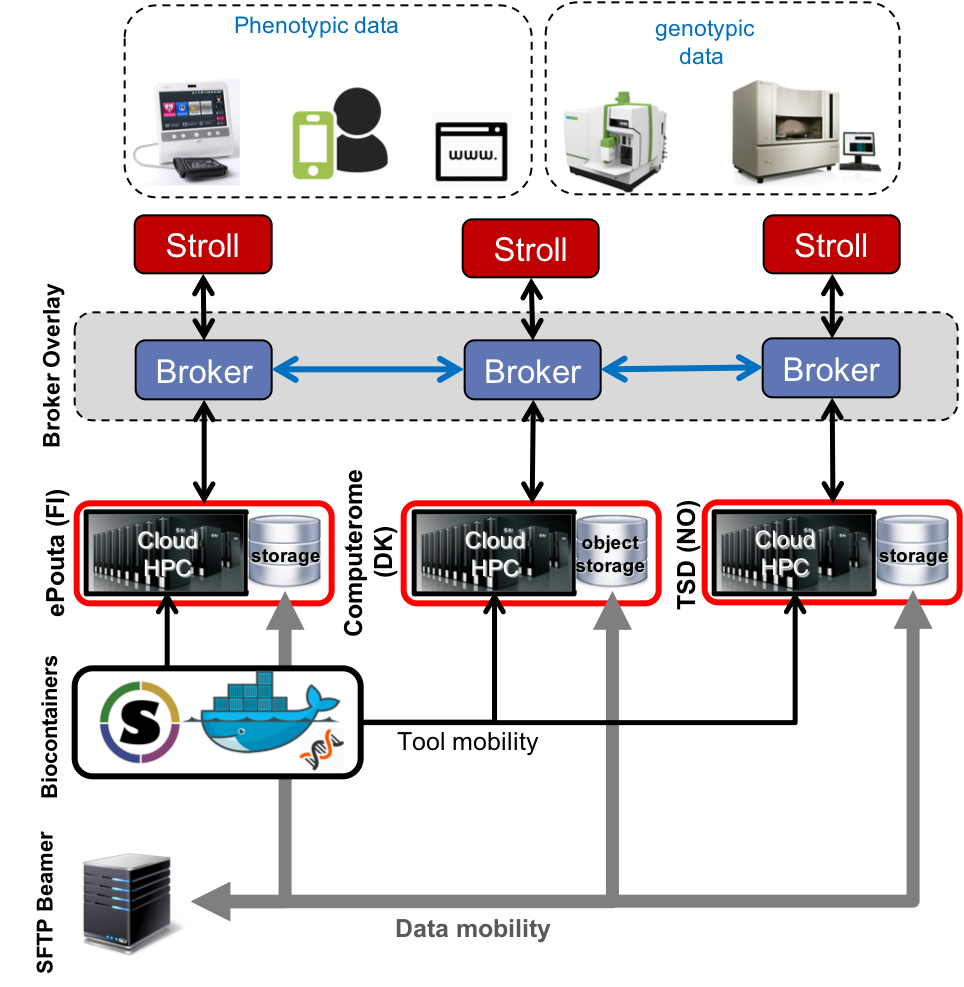
\includegraphics[width=.5\textwidth]{figures/tryggve-model}            
	\caption{Nordic sensitive data cloud federation}
	\label{fig:stroll-tryggve}
\end{figure}
